%%%%%%%%%%%%%%%%%%%%%%%%%%%%%%%%%%%%%%%%%%%%%%%%%%%%%%%%%%%%%%%%%%%%%%%%%%%%%%%%%%%%%%%%%%%%%%%%
%
% CS484 Written Question Template
%
% Acknowledgements:
% The original code is written by Prof. James Tompkin (james_tompkin@brown.edu).
% The second version is revised by Prof. Min H. Kim (minhkim@kaist.ac.kr).
%
% This is a LaTeX document. LaTeX is a markup language for producing 
% documents. Your task is to fill out this document, then to compile 
% it into a PDF document. 
%
% 
% TO COMPILE:
% > pdflatex thisfile.tex
%
% If you do not have LaTeX and need a LaTeX distribution:
% - Personal laptops (all common OS): www.latex-project.org/get/
% - We recommend latex compiler miktex (https://miktex.org/) for windows,
%   macTex (http://www.tug.org/mactex/) for macOS users.
%   And TeXstudio(http://www.texstudio.org/) for latex editor.
%   You should install both compiler and editor for editing latex.
%   The another option is Overleaf (https://www.overleaf.com/) which is 
%   an online latex editor.
%
% If you need help with LaTeX, please come to office hours. 
% Or, there is plenty of help online:
% https://en.wikibooks.org/wiki/LaTeX
%
% Good luck!
% Min and the CS484 staff
%
%%%%%%%%%%%%%%%%%%%%%%%%%%%%%%%%%%%%%%%%%%%%%%%%%%%%%%%%%%%%%%%%%%%%%%%%%%%%%%%%%%%%%%%%%%%%%%%%
%
% How to include two graphics on the same line:
% 
% \includegraphics[width=0.49\linewidth]{yourgraphic1.png}
% \includegraphics[width=0.49\linewidth]{yourgraphic2.png}
%
% How to include equations:
%
% \begin{equation}
% y = mx+c
% \end{equation}
% 
%%%%%%%%%%%%%%%%%%%%%%%%%%%%%%%%%%%%%%%%%%%%%%%%%%%%%%%%%%%%%%%%%%%%%%%%%%%%%%%%%%%%%%%%%%%%%%%%

\documentclass[11pt]{article}

\usepackage[english]{babel}
\usepackage[utf8]{inputenc}
\usepackage[colorlinks = true,
            linkcolor = blue,
            urlcolor  = blue]{hyperref}
\usepackage[a4paper,margin=1.5in]{geometry}
\usepackage{stackengine,graphicx}
\usepackage{fancyhdr}
\setlength{\headheight}{15pt}
\usepackage{microtype}
\usepackage{times}
\usepackage{booktabs}
\usepackage{listings}
% From https://ctan.org/pkg/matlab-prettifier
\usepackage[numbered,framed]{matlab-prettifier}
\lstdefinestyle{codestyle}{
	frame=single,
	basicstyle=\ttfamily\footnotesize,
	keywordstyle=\bfseries\color{magenta},
	commentstyle=\itshape\color{gray},
	stringstyle=\color{orange},
	numberstyle=\sffamily\scriptsize\color{gray},
	showspaces=false,
	showstringspaces=false,
	showtabs=false,
	tabsize=4,
	breakatwhitespace=false,
	breaklines=true,
	keepspaces=true,
	captionpos=b,
	numbers=left,
	numbersep=5pt}
\lstset{style=codestyle}
\frenchspacing
\setlength{\parindent}{0cm} % Default is 15pt.
\setlength{\parskip}{0.3cm plus1mm minus1mm}

\pagestyle{fancy}
\fancyhf{}
\lhead{Project Writeup}
\rhead{CS 484}
\rfoot{\thepage}

\date{}

\title{\vspace{-1cm}Homework 4 Writeup}


\begin{document}
\maketitle
\vspace{-3cm}
\thispagestyle{fancy}

\section*{Instructions}
\begin{itemize}
  \item Describe any interesting decisions you made to write your algorithm.
  \item Show and discuss the results of your algorithm.
  \item Feel free to include code snippets, images, and equations.

\end{itemize}

\section*{Harris Corner Detector}
\begin{lstlisting}[language=python]
    def get_interest_points(image, descriptor_window_image_width):
        
        gradient_filter_x = np.array([[-1, 0, 1]])
        gradient_filter_y = np.array([[-1], [0], [1]])

        # Compute gradients by convolving gradient filters with the image
        Ix = cv2.filter2D(src=img_gray, kernel=gradient_filter_x, ddepth=-1)
        Iy = cv2.filter2D(src=img_gray, kernel=gradient_filter_y, ddepth=-1)

        # Compute products of derivatives
        sigma = 1
        alpha = 0.05
        threshold = 0.01
        Ixx = cv2.GaussianBlur(Ix * Ix, (5, 5), sigma)
        Iyy = cv2.GaussianBlur(Iy * Iy, (5, 5), sigma)
        Ixy = cv2.GaussianBlur(Ix * Iy, (5, 5), sigma)
        cornerness = (Ixx*Iyy) - (Ixy**2) - alpha*((Ixx+Iyy)**2)
        corners = cornerness > threshold * cornerness.max()
        distance = 1

        #Non Max Suppression
        for i in range(distance, corners.shape[0] - distance):
            for j in range(distance, corners.shape[1] - distance):
                if corners[i, j]:
                    local_max = cornerness[i - distance:i + distance + 1, j - distance:j + distance + 1].max()
                    if cornerness[i, j] != local_max:
                        corners[i, j] = False

        # Getting the coordinates of corners
        y, x = np.where(corners)
        return x, y
\end{lstlisting}

\begin{enumerate}
    \item \textbf{Obtaining Image Gradient} First, I obtained the image gradient for horizontal and vertical directions. To do this, I made a kernel of $\left[-1,0,1\right]$ and ${\left[ -1,0,1 \right]}^T$ 
    For each kernel, I applied to the image with cv2.filter2D function. This produces $I_{x}$ and $I_{y}$, each a gradient array for x direction and y direction.
    
    \item \textbf{Calculating Cornerness and extracting corner} With Harris Corner Detector equation and the gradient, I produced the cornerness value. For hyperparameter sigma, alpha, and corner threhold was used.
    
    $threshold\times(biggest\_cornerness\_value)$. If I increase the threshold, more corner points were extracted. I choosed the appropriate threshold based on the given corner points count for each images.
    \item \textbf{Non-Max Suppression} To apply non-max suppression, I iterated through the corner matrix, and for each pixels that are chosen for corner I checked out if it is the local maximum in $3\times3$ neighborhood.  If it is not, I excluded it from the corner list.
    
    
\end{enumerate}

\section*{SIFT Feature Descriptor}
\begin{lstlisting}[language=python]
    def get_descriptors(image, x, y, descriptor_window_image_width):
        
        x = np.round(x).astype(int)
        y = np.round(y).astype(int)

        num_bins = 8
        window_width = descriptor_window_image_width // 4  # width of the 4x4 cells in a window

        descriptors = np.zeros((len(x), 128))  # 128 = 16 histograms * 8 bins per histogram

        gradient_filter_x = np.array([[-1, 0, 1]])
        gradient_filter_y = np.array([[-1], [0], [1]])

        # Compute gradients by convolving gradient filters with the image
        dx = cv2.filter2D(src=image, kernel=gradient_filter_x, ddepth=-1)
        dy = cv2.filter2D(src=image, kernel=gradient_filter_y, ddepth=-1)
        magnitude = np.sqrt(np.add(np.square(dx), np.square(dy)))
        orientation = np.arctan2(dy, dx) * (180 / np.pi) % 360

        gaussian_window = cv2.getGaussianKernel(descriptor_window_image_width, descriptor_window_image_width / 2)
        gaussian_window = gaussian_window * gaussian_window.T

        for idx in range(len(x)):
            xi=x[idx]
            yi=y[idx]
            # Ensure the window is fully within the image bounds
            min_x = max(xi - window_width * 2, 0) 
            max_x = min(xi + window_width * 2, image.shape[1])
            min_y = max(yi - window_width * 2, 0)
            max_y = min(yi + window_width * 2, image.shape[0])

            window_magnitude = magnitude[min_y:max_y, min_x:max_x]
            window_orientation = orientation[min_y:max_y, min_x:max_x]
            # Apply the Gaussian window
            weight_window_magnitude = window_magnitude * gaussian_window[min_y - yi + window_width * 2:max_y - yi + window_width * 2,
                                                                        min_x - xi + window_width * 2:max_x - xi + window_width * 2]

            descriptor_vector = np.zeros((4, 4, num_bins))

            for i in range(4):
                for j in range(4):
                    subregion_w_mag = weight_window_magnitude[window_width*i:window_width*(i+1), window_width*j:window_width*(j+1)].flatten()
                    subregion_orientation = window_orientation[window_width*i:window_width*(i+1), window_width*j:window_width*(j+1)].flatten()

                    hist, _ = np.histogram(subregion_orientation, bins=num_bins, range=(0, 360), weights=subregion_w_mag)
                    descriptor_vector[i, j, :] = hist

            # Normalize the descriptor
            descriptor_vector = descriptor_vector.flatten()
            descriptor_vector /= (np.linalg.norm(descriptor_vector) + 1e-7) # Preventing division by zero

            # Clip values to 0.2 and re-normalize
            descriptor_vector = np.clip(descriptor_vector, 0, 0.2)
            descriptor_vector /= (np.linalg.norm(descriptor_vector) + 1e-7) 

            descriptors[idx, :] = descriptor_vector

        return descriptors
\end{lstlisting}

\begin{enumerate}
    \item \textbf{Calculating Image magnitude and orientation} First, for computational efficiency, I pre-calculated the magnitude and orientation of feature vectors. To do this, with the same way used in feature detection I obtained the gradient and calculated magnitude and orientation.
    \item \textbf{Gaussian Window} Furthermore I calculated the gaussian kernel with the size of the descriptor window, to assign weights to the pixel values in the descriptor.
    \item \textbf{Calculating descriptor} Iterating through the corner points given, I initialized the descriptor vector by applying the pre-calculated gaussian window to the local magnitude array. I also considered the boundary condition, so started from the half size of the descriptor window.
    \item \textbf{Creating Histogram} For each $4\times4$ cell in the descriptor window, cacluated the magnitude and orientation of the subregion. Then, with np.histogram function made a histogram for each subregions. This leads to $4\times4\times8=128$ dimensions feature descriptor
    \item \textbf{Normalization and Clipping} Finally, I normalized the descriptor and clipped the values to 0,2; then re-normalized to obtain the final descriptor.
\end{enumerate}

\section*{Feature Matching}
\begin{lstlisting}[language=python]
    def match_features(features1, features2):
        matches = []
        confidences = []
        ratio = 0.8

        for i in range(features1.shape[0]):

            distances = np.sqrt(np.square(np.subtract(features1[i, :], features2)).sum(axis=1))

            sorted_indices = np.argsort(distances)
            closest_neighbor_index = sorted_indices[0]
            second_closest_neighbor_index = sorted_indices[1]

            nn_distance_ratio = distances[closest_neighbor_index] / distances[second_closest_neighbor_index]

            if nn_distance_ratio < ratio:
                matches.append([i, closest_neighbor_index])
                confidences.append(1.0 - nn_distance_ratio)

        matches = np.array(matches)
        confidences = np.array(confidences)

        sorted_indices = np.argsort(confidences)
        matches = matches[sorted_indices]
        confidences = confidences[sorted_indices]

        return matches, confidences
\end{lstlisting}
\begin{enumerate}
    \item \textbf{Calculating Nearest Neighbor} For descriptor vectors obtained from SIFT, I applied Nearest neighbor with Euclidean distance to match the good features. After calculating the Euclidean distance between the feature of two images, I sorted the vectors in order of distance. Then, I calculated the ratio between first and second nearest neighbor's distance.
    \item \textbf{Applying Threshold to pick the feature point} I applied threshold of 80\%, and selected the matches bigger than the threshold for good matches and appended in the array.
    \item \textbf{Sorting} Finally, I cacluated the confidence value by extracing the ratio from 1, and sorted all the indices with confidence.
\end{enumerate}

\section*{Feature Matching Results}

    \begin{figure}[htb!]
        \centering
        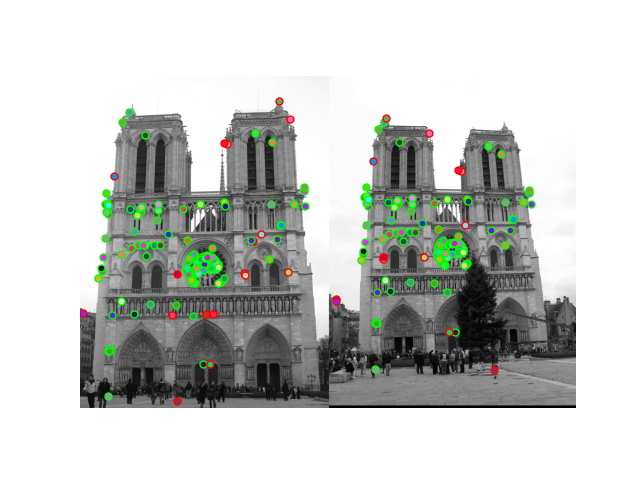
\includegraphics[width=15cm]{../eval_ND.png}
        \caption{Notre Dame. In this image, with 160 submitted matches the accuracy was \textbf{89.31\%} and for 100 matches in decreasing confidence the accuracy was \textbf{91\%}.}
        \label{fig:result1}
    \end{figure}
    
    \begin{figure}[htb!]
        \centering
        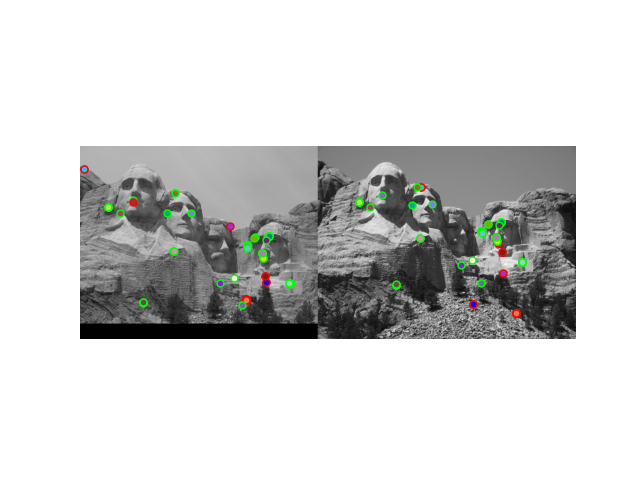
\includegraphics[width=15cm]{../eval_MR.png}
        \caption{Mount Rushmore. In this image, with 226 submitted matches the accuracy was \textbf{97.35\%} and for 100 matches in decreasing confidence the accuracy was \textbf{97.00\%}.}
        \label{fig:result2}
    \end{figure}
\clearpage    
    \begin{figure}[htb!]
        \centering
        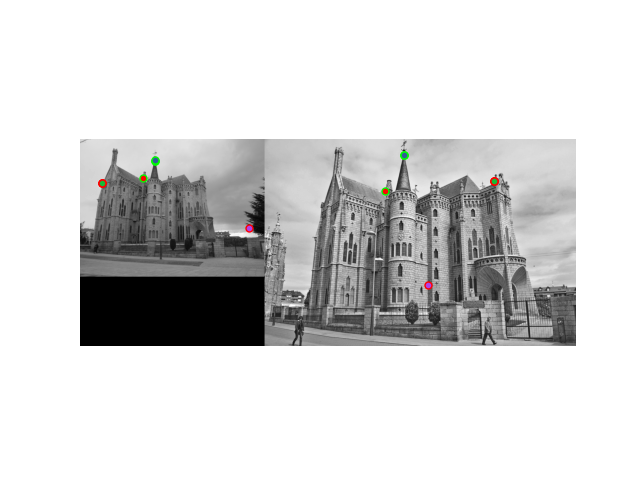
\includegraphics[width=15cm]{../eval_EG.png}
        \caption{Episcopal Gaudi. In this image, with 5 submitted matches the accuracy was \textbf{60.00\%} and for 100 matches in decreasing confidence the accuracy was \textbf{3.00\%}.}
        \label{fig:result3}
    \end{figure}
    We can notice that the accuracy dropped in this image. I think this is because in this picture the brick pattern in the wall makes ambiguity between the feature points; we can't easily distinguish the feature points on those repitive patterns with nearest neighbor algorithm.
\clearpage
\section*{Normalized Patch Descriptor VS SIFT Descriptor}
This is the normalized patch descriptor that I implemented at first.
\begin{lstlisting}[language=python]
    def get_descriptors(image, x, y, descriptor_window_image_width):
        x = np.round(x).astype(int)
        y = np.round(y).astype(int)

        patch_half_width = descriptor_window_image_width // 2

        descriptors = np.zeros((len(x), descriptor_window_image_width ** 2))

        for idx in range(len(x)):
            xi = x[idx]
            yi = y[idx]

            min_x = max(xi - patch_half_width, 0)
            max_x = min(xi + patch_half_width, image.shape[1])
            min_y = max(yi - patch_half_width, 0)
            max_y = min(yi + patch_half_width, image.shape[0])

            patch = image[min_y:max_y, min_x:max_x]
            resized_patch = cv2.resize(patch, (descriptor_window_image_width, descriptor_window_image_width))

            patch_descriptor = resized_patch.flatten()
            patch_descriptor = patch_descriptor / np.linalg.norm(patch_descriptor)

            descriptors[idx, :] = patch_descriptor

        return descriptors
\end{lstlisting}
I simply made a patch around each feature points from Harris corner detector and normalized them and used them as the feature vector.
For Noter Dame image, with this descriptor and all the other code identical, showed \textbf{78.05\%} accuracy in all matches and \textbf{64\%} accuracy for 100 matches by decreasing confidences, compared to \textbf{89.31\%} and \textbf{91\%} of SIFT descriptor.






\end{document}
